\documentclass{article}
\usepackage[utf8]{inputenc}
\usepackage[left=1in,right=1in,top=1in,bottom=1in]{geometry}
\usepackage{authblk}
\usepackage{blindtext}
\usepackage{graphics}
\usepackage{graphicx}
\usepackage{caption}
\usepackage{multirow}
\date{}
\begin{document}
\title{\LARGE \bf
How synthetic data can enhance the performance of machine learning models in the healthcare domain: A heart murmur detection case study}


\author[1]{Alireza Rafiei\thanks{alireza.rafiei@emory.edu}}

\affil[1]{Department of Computer Science and Informatics, Emory University, Atlanta, GA}

\maketitle

\begin{abstract}

Heart murmurs require timely detection and accurate diagnosis to facilitate effective clinical decision-making. Machine learning approaches are replacing traditional methods to detect heart murmurs to prevent variability and subjectivity in clinical decisions and the need for experienced healthcare professionals. However, the scarcity of large-scale and well-labeled data for heart murmur detection poses a significant challenge to the development of robust and accurate automated models. This technical report investigates the role of synthetic data in enhancing the performance of machine learning models for murmur detection. In this regard, we first manipulated 3,163 publicly available phonocardiography (PCG) records from the CirCor DigiScope PCG dataset to generate synthetic data. We added background noise that mimicked real hospital sounds and modified the signal-to-noise ratio of the records to create this synthetic data. Subsequently, we developed four distinct machine learning models, training each one using the original dataset and then using a combination of the original and synthetic datasets. The developed InceptionTime model achieved a 0.774 accuracy and 0.691 AUC once training on the combined data as the best scenario. Our findings demonstrate that generating synthetic data for the development of machine learning algorithms can improve their performance.

\end{abstract}



\section{Introduction}
The healthcare sector generates and accumulates a vast amount of data every day. This data is critical for medical research, diagnosis, and treatment planning. With the advent of machine learning, this data has become even more valuable for improving patient outcomes and reducing healthcare costs \cite{obermeyer2016predicting}. However, the effectiveness of these cutting-edge technologies is contingent upon the availability and quality of data used for model training \cite{rajkomar2019machine}. In many cases, the datasets available for training machine learning models are insufficient, imbalanced, deficit, and biased, which can hinder progress in harnessing the full potential of machine learning for healthcare \cite{johnson2016machine,dash2019big}. In addition, the sensitive nature of health-related information, along with strict regulatory and security requirements, makes it difficult to obtain and use healthcare data machine learning model development \cite{winter2019governance}. These necessitate the exploration of alternative data generation methods, such as synthetic data, to circumvent these obstacles and propel the field forward.

\par In light of these challenges, synthetic data generation has emerged as a promising avenue for circumventing the limitations associated with real-world healthcare data. By generating new data replicating real-world data's essential characteristics, but with additional variations, synthetic data can facilitate the development of robust and reliable machine learning models in healthcare \cite{chen2021synthetic,murtaza2023synthetic} The adoption of synthetic data in the healthcare domain can also alleviate several pressing concerns, including protecting sensitive patient information and adhering to stringent regulations \cite{gonzales2023synthetic} Additionally, synthetic data generation techniques can contribute to overcoming the challenges posed by the heterogeneous nature of healthcare data since it can be generated in a harmonized format, thereby simplifying the data preprocessing and integration tasks essential for model training. Moreover, synthetic data can help address data quality, completeness, and representation issues by generating balanced and comprehensive datasets that reduce biases and improve the generalizability of machine learning models \cite{das2022conditional}.

\par Heart murmurs, characterized by abnormal heart sounds resulting from turbulent blood flow within the cardiac chambers or through the valves, have garnered significant attention in the medical community due to their potential implications for cardiovascular health. While some murmurs may be benign or physiological, others can indicate underlying pathological conditions that necessitate prompt diagnosis and intervention. The accurate identification and classification of heart murmurs are crucial for guiding clinicians in making informed decisions regarding patient care and management. Physicians typically detect a heart murmur when listening to the heart using a stethoscope or pre-recorded phonocardiography (PCG) of patients. A PCG is a graphical representation of the acoustic signals produced by the heart, displaying the amplitude and frequency of heart sounds and murmurs over time. This technique is particularly useful for detecting, characterizing, and monitoring heart murmurs, as it allows for a more detailed and quantitative assessment of the acoustic properties of these abnormal sounds.

\par In order to develop a dependable machine learning model suitable for real-world applications, a substantial volume of data is necessary \cite{alom2019state}. However, the availability of annotated PCG data specific to certain conditions, such as heart murmurs, remains limited. In addition, the lack of a universally accepted standard for PCG data collection, storage, and analysis further exacerbates inconsistencies and challenges when comparing and integrating data from disparate sources. To overcome these issues, the prospective machine learning model should be trained using a diverse range of data sources. Synthetic PCG data can play a significant role in supplying adequate data to establish a generalizable and robust automated heart murmur detection model.


\par In this study, we generated synthetic PCG records, which were able to preserve the subtle patterns of the original data, thereby providing additional training data for machine learning models to enhance their ability to detect heart murmurs with improved performance metrics. To achieve this, we initially designed two distinct filters to simulate the real hospital environment and the inherent instrument noise. Subsequently, we divided each of the original and generated synthetic records into smaller sub-segments and represented each segment as a two-dimensional image. Finally, we developed and evaluated four machine learning models using the original and synthetic data separately.


\section{Materials and methods}
\subsection{The PCG dataset}
The dataset utilized in this study is the CirCor DigiScope PCG dataset \cite{Reyna2022.08.11.22278688,oliveira2021circor}, which is a collection of heart sound signals gathered over two mass screening campaigns in Paraiba, Brazil, from 2014-2015. This dataset was primarily created to study and classify cardiac diseases in a pediatric and pregnant population. Unlike other PCG datasets \cite{clifford2016classification,kazemnejad2021open}, which usually involve a single recording from a single location for each patient, the CirCor dataset includes multiple PCG recordings from various auscultation locations, including pulmonary valve, aortic
valve, mitral valve, and tricuspid valve. Nonetheless, some patients had fewer than four recordings, while a few had multiple recordings from the same location. The recordings were obtained sequentially and may vary in number, location, and duration across patients.

\par The dataset contains 5272 PCG recordings (3163 recordings are publically available) taken from 1568 patients, with an average age of 6.1 (±4.3) years and a range of 0 to 21 years. The PCGs were captured at a sampling rate of 4000 Hz using the DigiScope Collector technology, which is part of the Littmann 3200 stethoscope. The shortest and longest recording durations are 4.8 s and 80.4 s, respectively. The average heart rate is 102 (±20) beats per minute (bpm), with a range of 47 to 193 bpm.

\par The annotations in the dataset provide detailed information about the characteristics of murmurs. They indicate whether a patient has a murmur and present a complete description of the event, including its location, quality, type, shape, pitch, timing, and intensity grade. The expert annotator has also labeled each record as either having a murmur present, absent, or unknown (for low-quality records).


\subsection{Pre-processing}
The PCG recordings were divided into segments of 3 seconds each, using a sliding window technique without overlapping. To represent each segment, a two-dimensional image was created using the logarithmic Mel spectrogram technique. The spectrogram was calculated using the same parameters as in the previous study \cite{elola2022beyond}, including Hamming windows of 25 milliseconds with 50\% overlap and FFT of 512 points in the frequency range 0-800Hz. This frequency range was chosen because murmurs are not typically present in higher frequencies \cite{mcgee2018auscultation}. After applying the Mel filter bank, 32 values were obtained for each frame. Figure \ref{fig:PP} demonstrates the applied pre-processing workflow on the raw PCG data.

\par The final representation of every 3-second heard signal recording segment is a 32x240 matrix. The Mel spectrogram depiction of the PCG was opted for this study since it is widely recognized by the audio processing community for its similarity to human hearing. To train the machine learning models, labels were generated for the recording level from the available patient-level label. In this regard, the labels for each recording were assumed to be the same as the patient-level label. The analysis windows for each recording then adopted the label assigned at the recording level.


\begin{figure}
\centering
    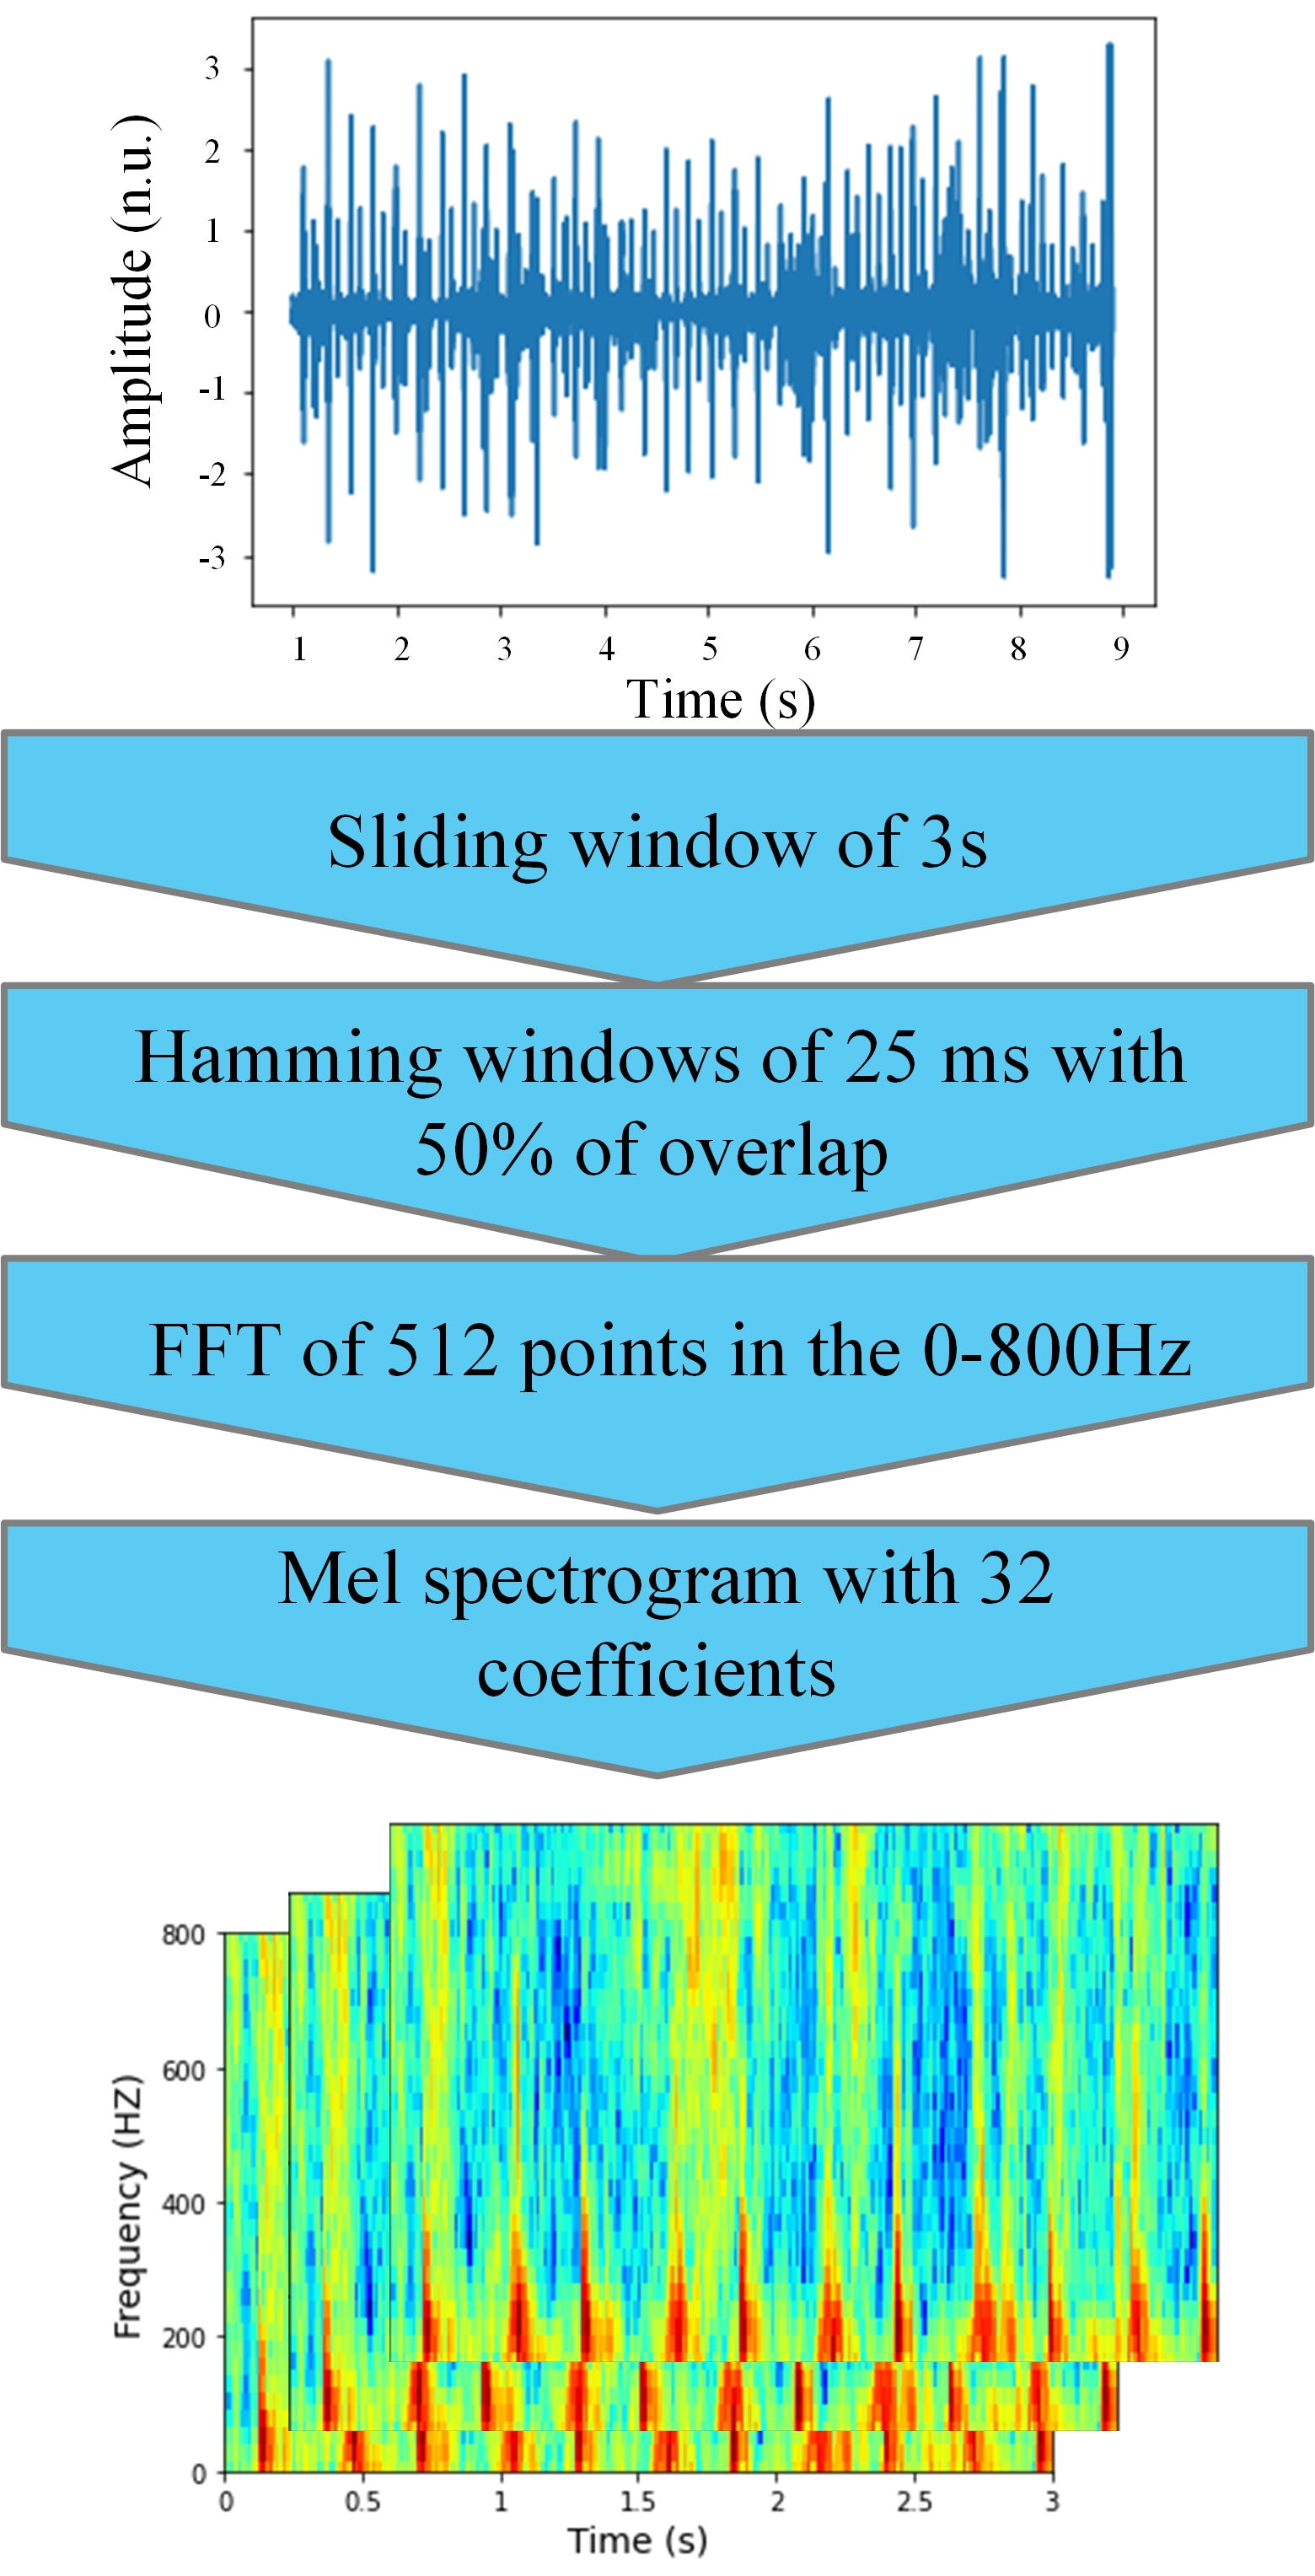
\includegraphics[width=0.4\textwidth]{Documents/preprecessing.jpg}
    \caption{Pre-processing workflow.}
    \label{fig:PP}

\end{figure}


\subsection{Forward modeling}
We developed two distinct filters to generate synthetic data with the aim of simulating the real-world environment of the hospital and the inherent noise of recording instruments. The first filter is designed to dilute the PCG records with background audio sounds and white Gaussian noise. This filter utilizes a wide variety of environmental sounds from different scenarios to introduce audio interference into the PCG records to simulate the real circumstance of the hospital. White noise is a type of random noise that follows a Gaussian distribution with a mean of zero and equal power across all frequencies and aim to simulate the recording instruments' noise. The user can specify the desired signal-to-interference ratios (SIRs) for the background audio and signal-to-noise ratios (SNRs) for the white noise, allowing them to control the level of noise added. After the noise has been introduced, the noisy PCG signals are processed using variable group delay filters. These filters are designed to alter the phase characteristics of the signals without significantly affecting their amplitude. We set the SIR to -15 and 15, and SNR to 15 to produce 2581 numbers of synthetic data using this filter. The second filter processed the PCG data by introducing noise at varying SNRs and subsequently filtering the noisy signals using a bypass innovations filter. The noisy signals are then filtered and the power of the filtered signals is normalized to that of the original signal. To ensure that the processed signals maintain their amplitude range, the filter corrects any positive or negative clipping that may have occurred during filtering. We have set the SNR to -15 and 15 to produce 2581 numbers of synthetic data using this filter. The synthetic data filters were implemented in MATLAB 2022b. Figure \ref{fig:GD} illustrates a random example of the absence of murmured, presence of murmur, and unknown records for the original and two generated synthetic datasets.


\par We calculated the results for the Kullback-Leibler divergence, total variation distance, and Hellinger distance for the two synthetic datasets generated from the original dataset to quantify the dissimilarity between two probability distributions, with lower values indicating a closer resemblance (Tabel \ref {tab:GD}). Upon analyzing the KL divergence values of the two synthetic datasets generated from the original dataset, the amplitude phase altering dataset (0.0957) was more similar to the original dataset than the randomized group delays dataset (0.6685), indicating that the method employed for the amplitude phase altering data generation better preserves the underlying distribution. Similarly, amplitude phase altering dataset (0.0957) had a lower total variation distance compared to the randomized group delays dataset (0.1877), suggesting that this synthetic dataset more closely approximates the original dataset in terms of the probability distribution. The amplitude phase altering dataset also exhibited a smaller Hellinger Distance (0.1010) than the randomized group delays (0.2493), reinforcing that this data was more similar to the original dataset. Across all three measures, synthetic data of the amplitude phase altering technique consistently resembled the original dataset more closely than synthetic data of the randomized group delays approach. This suggested that the first data generation method was more effective in preserving the original data distribution.

\par The probability density function (PDF) and cumulative density function (CDF) are depicted in Figures \ref{fig:PD} and \ref{fig:CP}, respectively, representing the power spectra for all recordings following the pre-processing steps. The PDF was calculated to display the relative frequency of each possible power spectrum in the original dataset and the two synthetically generated datasets. The original dataset and the amplitude phase-adjusted dataset exhibited nearly normal distributions, whereas the random group delays dataset demonstrated a skewed distribution across power spectra. The CDF plot represented a smooth, increasing, sigmoid-shaped curve for all three datasets. As clearly can be seen, the probability of a higher power spectrum occurrence in the randomized group delay dataset was higher than in the two other datasets. Of note, the cumulative probability of a 60 dB power spectrum is less than 0.4 for the randomized group delay dataset, whereas it exceeds 0.6 for both the original and amplitude phase-adjusted datasets.


\begin{table}
\centering
\caption{Similarity analysis between the two generated synthetic datasets and the original dataset.}
\label{tab:GD}
\begin{tabular}{|l|c|c|c|}
\hline
Dataset                  & Kullback-Leibler divergence                & Total Variation Distance & Hellinger Distance \\ \hline
Amplitude phase altering & 0.0957                                     & 0.0696                   & 0.1010             \\ \hline
Randomized group delays   & 0.6685  & 0.1877                   & 0.2493  \\ \hline 

\end{tabular}
\end{table}

\begin{figure}
\centering
    \includegraphics[width=1\textwidth]{Documents/Generated data.jpg}
    \caption{Random examples of the three classes of murmur records for different datasets.}
    \label{fig:GD}

\end{figure}


\begin{figure}
\centering
    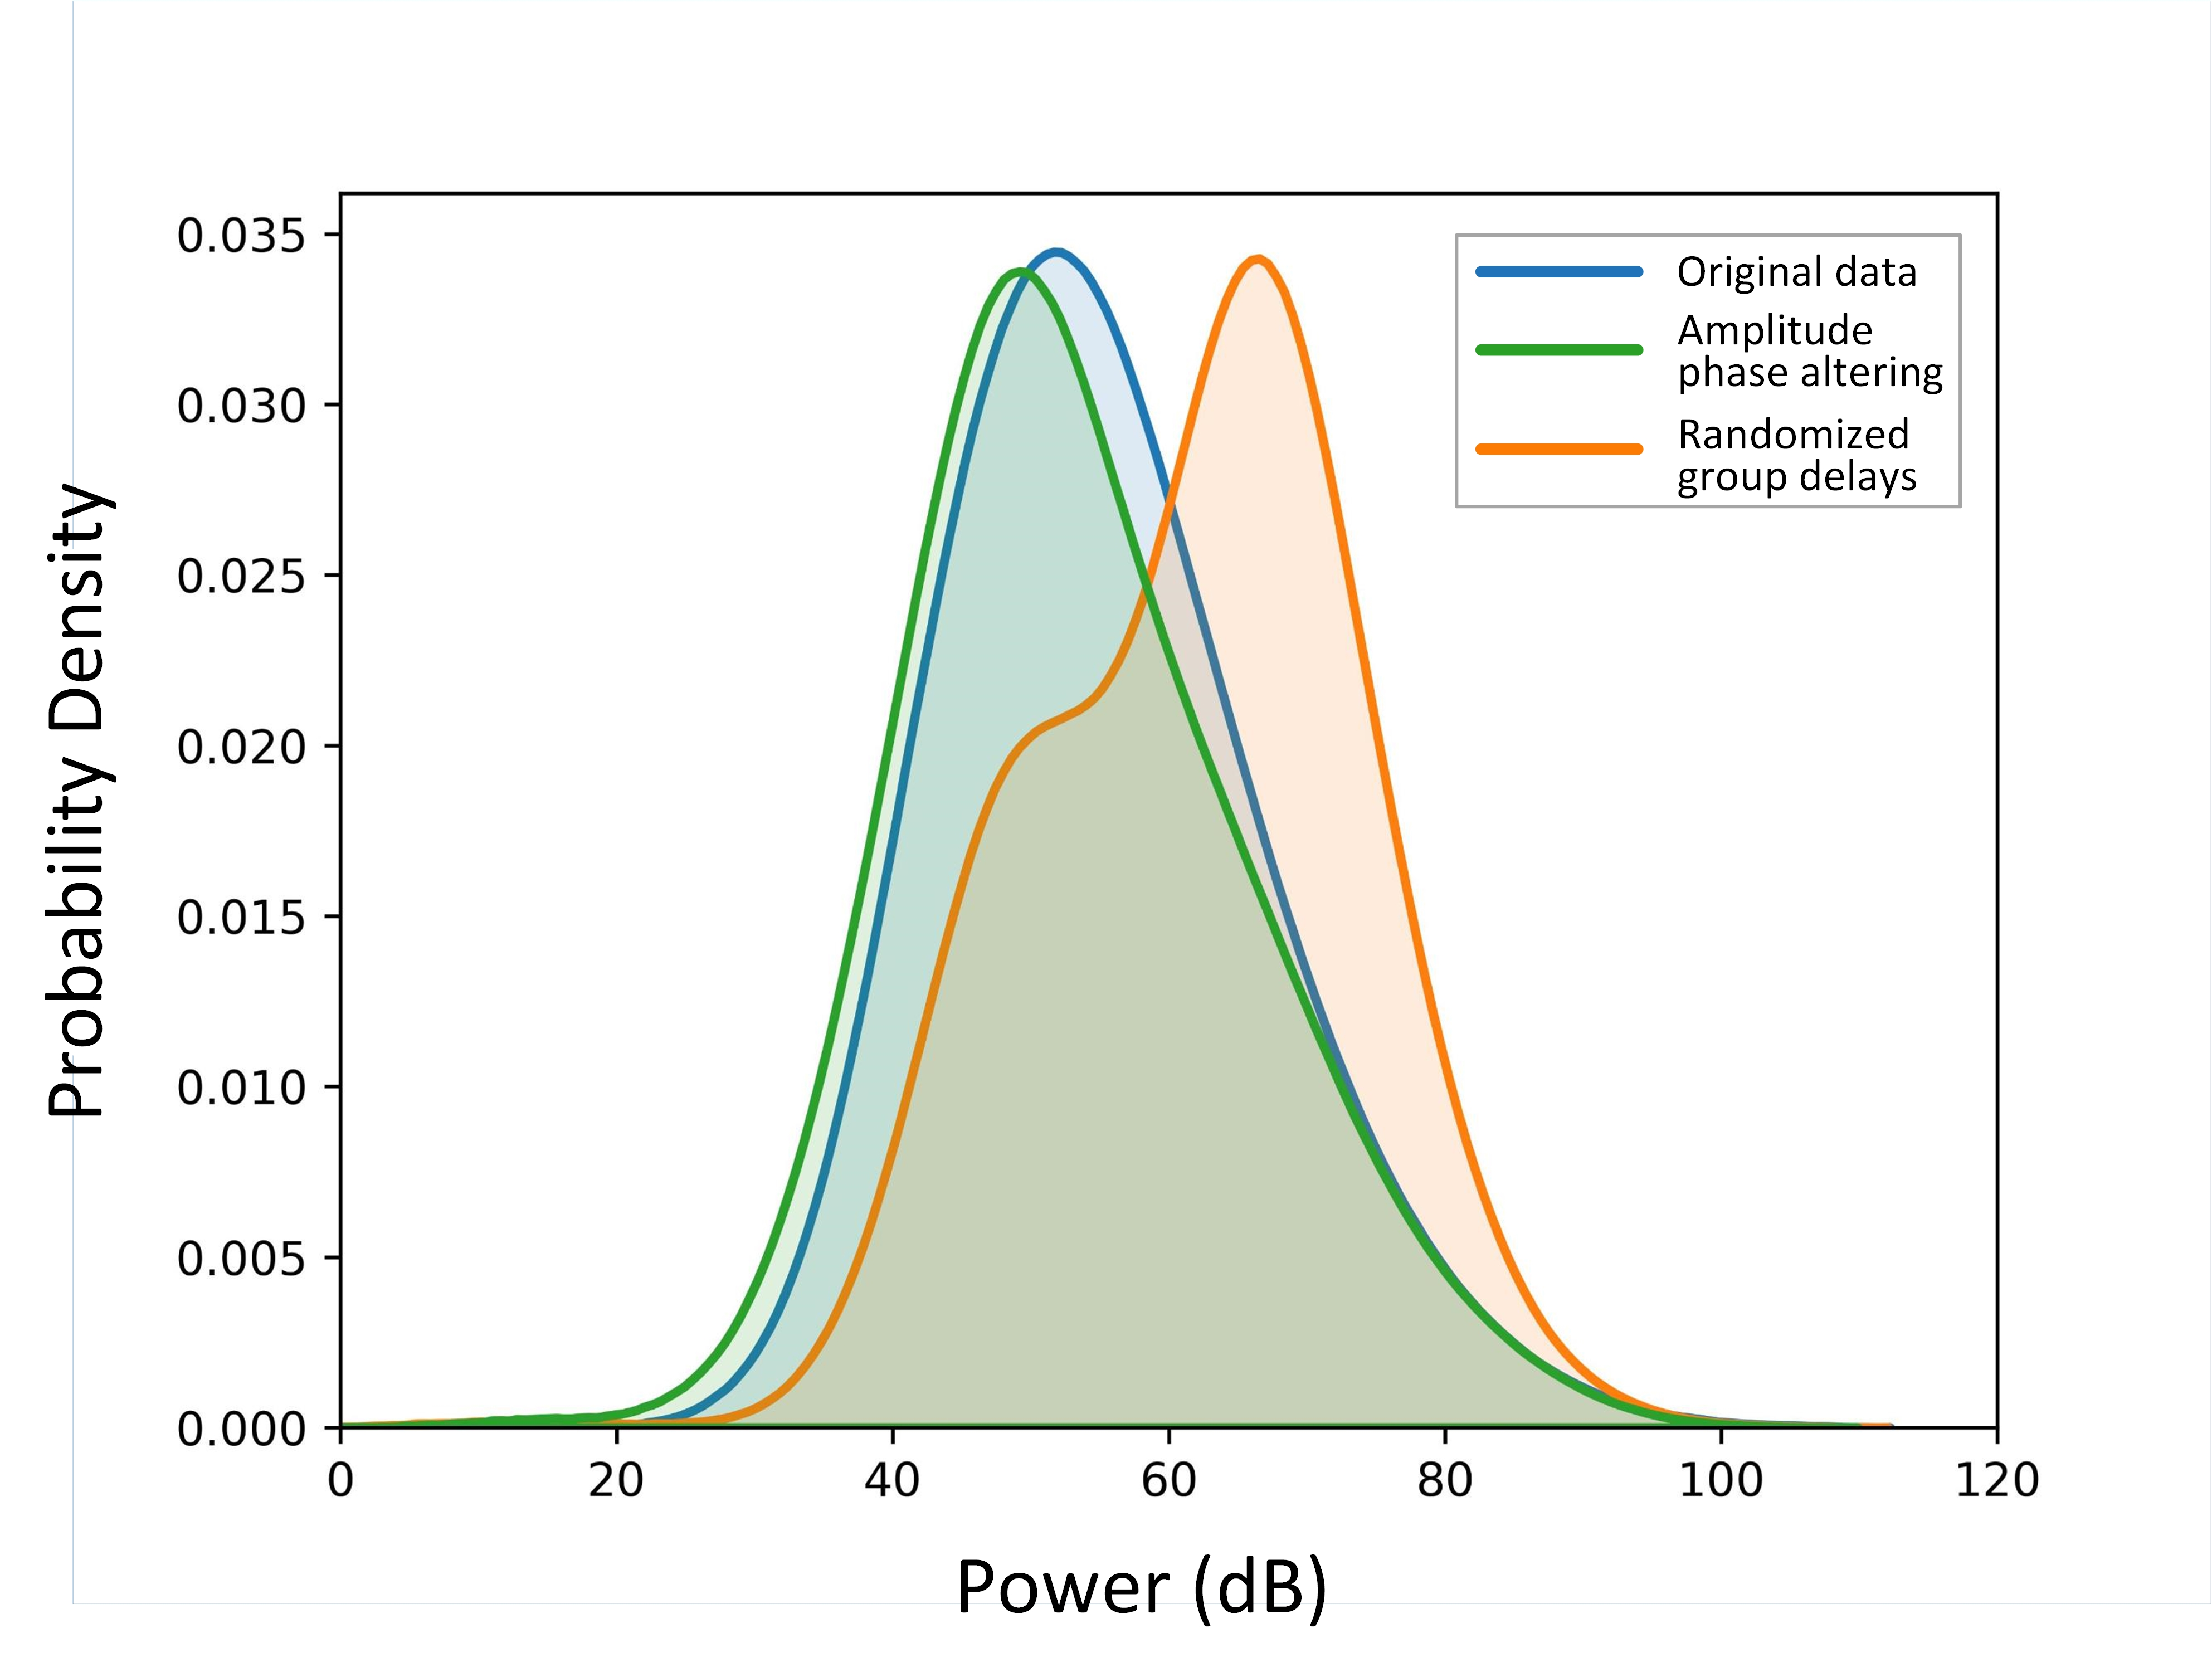
\includegraphics[width=0.6\textwidth]{Documents/pd.jpg}
    \caption{Probability density of power spectra across all recordings for the three datasets.}
    \label{fig:PD}

\end{figure}


\begin{figure}
\centering
    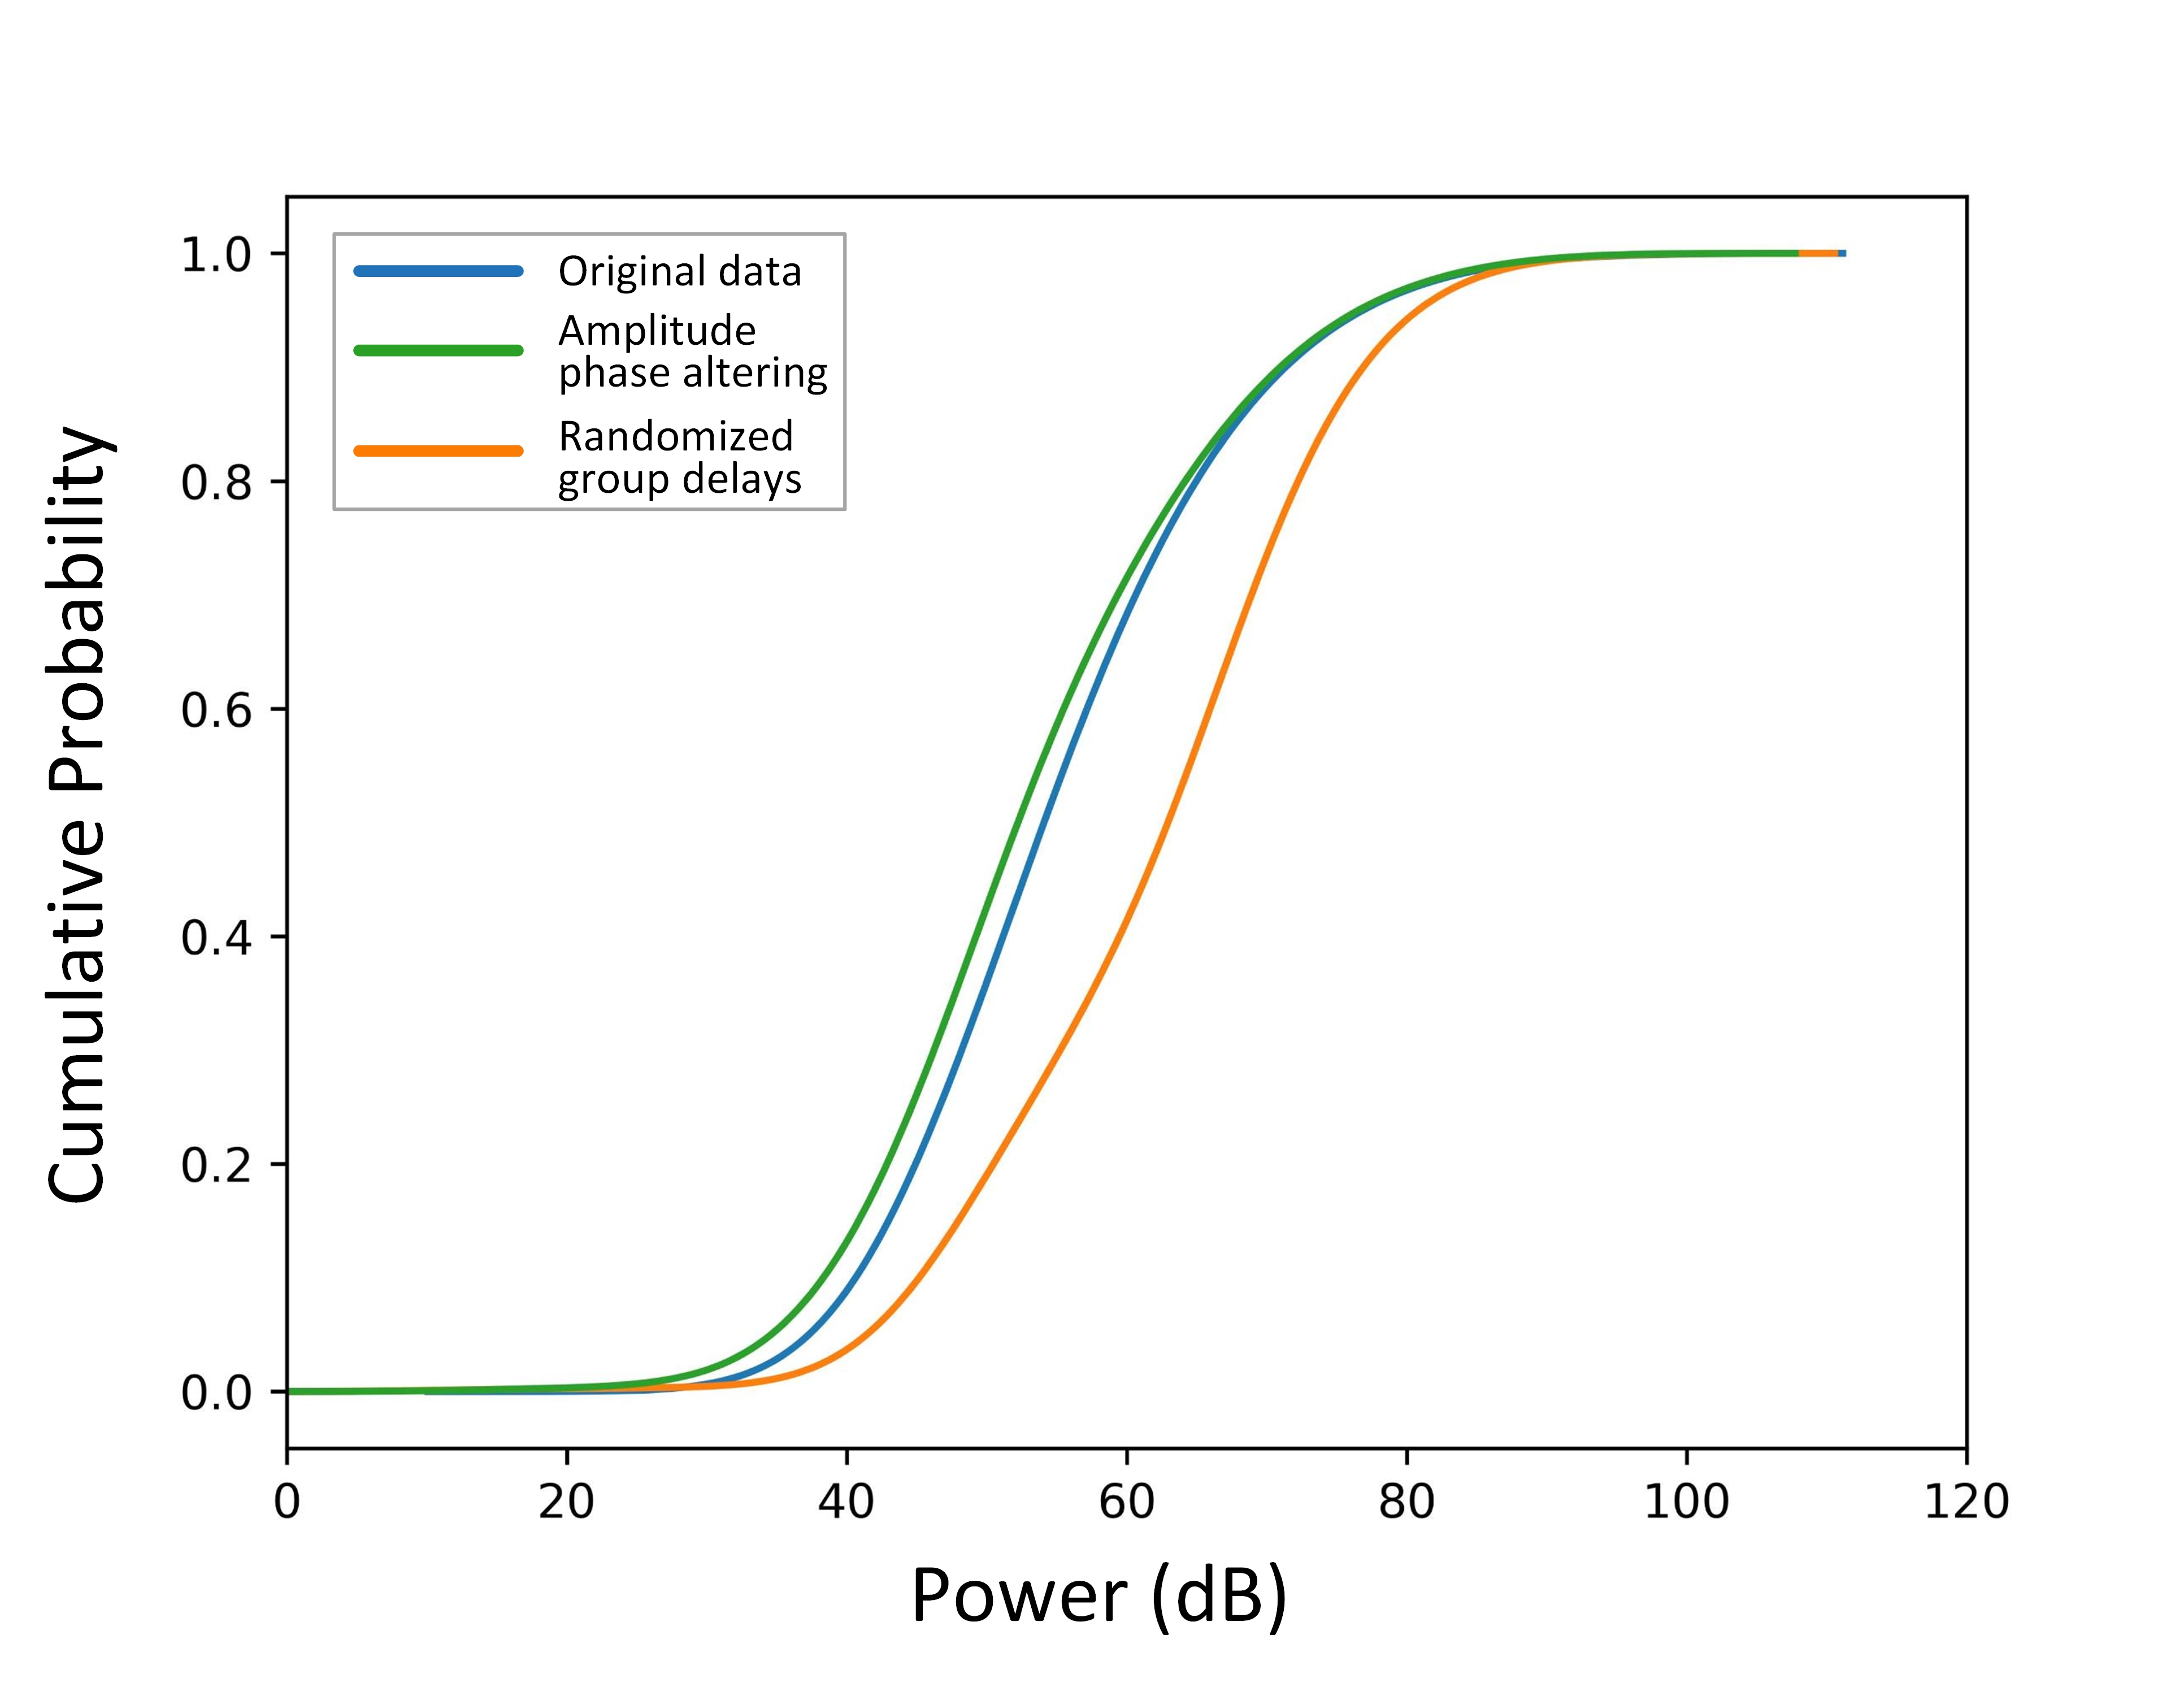
\includegraphics[width=0.6\textwidth]{Documents/cp.jpg}
    \caption{Cumulative probability of power spectra across all recordings for the three datasets.}
    \label{fig:CP}

\end{figure}

\subsection{Learning models}
In order to assess the effectiveness of the synthetic data approach, we examined the performance metrics of four distinct machine learning models: a basic two-layer Convolutional Neural Network (CNN), DeepConvNet, VGG-16, and InceptionTime. The simple CNN model comprising two CNN layers, followed by a max-pooling layer and a fully connected layer, was utilized as a baseline model. Additionally, we implemented both shallow and deep pre-trained CNN models by freezing the convolutional blocks and appending new fully connected layers.

\par The DeepConvNet model \cite{schirrmeister2017deep} proposed to enhance the analysis of electroencephalogram (EEG) signals by leveraging the hierarchical structure of CNNs. DeepConvNet's architecture consists of alternating convolutional and pooling layers, followed by fully connected layers and a final softmax layer for classification. We kept the same number of fully-connected layers and neurons (2 layers with 1000 and 500 neurons, respectively) of the proposed architecture for training the model. The VGG-16 architecture has been widely adopted and recognized as a seminal work for its remarkable performance in image classification tasks \cite{simonyan2014very}. It comprises 16 weighted layers, including 13 convolutional layers and three fully connected layers. We froze the convolutional layers and retrained three fully connected layers with 1024, 256, and 64 neurons and a dropout rate of 20\%. InceptionTime is a sophisticated ensemble of CNNs designed to adeptly learn and distinguish between local and global shape patterns \cite{rafiei2022automated}. The architecture comprises six Inception blocks, each containing parallel convolutional layers with three kernel sizes, allowing the model to learn different time-scale features simultaneously. The outputs of these parallel layers are concatenated and passed through a residual connection, mitigating the vanishing gradient problem. In the training phase, we set the bottleneck hyperparameter to 32. The developed machine learning models were implemented in Python 3.8.8 using Keras framework 2.11.0 with Tensorflow 2.11.0 as the backend.


\section{Results}
To train and assess the performance of the machine learning models, we partitioned 60\% of the original dataset into a training set. Following this, we generated synthetic datasets and pre-processed all available data to create two-dimensional images. Each of the four machine learning models was trained twice: first, using only the original training set, and second, using a combination of the original training set and the generated synthetic datasets. We calculated the area under the ROC curve (AUC), accuracy, F1-score, sensitivity, and specificity of the models on the test set (Table \ref{tab:PF}).

\par The DeepCovNet model was not able to show an acceptable performance as it could not learn the desirable patterns to distinguish murmur cases from the PCG records. Its performance remained roughly the same when trained on both the original and synthetic datasets, with an AUC of approximately 0.5, which is equivalent to random guessing. In contrast, the developed CNN showed a significant improvement when trained on the synthetic data, achieving an AUC of 0.563 and a sensitivity of 0.382, as opposed to an AUC of 0.526 and a sensitivity of 0.336 when trained on the original data. The VGG-16 had roughly the same accuracy, f1-score, and sensitivity when trained on the original data, but there was an increase in specificity metrics when it was trained on the synthetic data. The InceptionTime model outperformed all other models in both training scenarios. It achieved an AUC of 0.673 and an accuracy of 0.769 when trained on the original data, while it reached an AUC of 0.691 and an accuracy of 0.774 when trained on the synthetic data.

\par Figure \ref{fig:ROC} depicts the ROC curves for all machine learning models under both training scenarios. The lighter curves represent the test results of various learning models trained on the original and synthetic data, while the bold curve illustrates the average results of the four machine learning models across the two training scenarios. As can be clearly observed, the average performance of the models trained using synthetic data is marginally superior to that of their original counterparts. Figure \ref{fig:ROCs} illustrates the distinct ROC curves for each of the developed machine learning models. The DeepConvNet and VGG-16 models exhibit remarkably similar curve trajectories, whereas the differences between the two training scenarios for the CNN and InceptionTime models are more pronounced.

\begin{table}[]
\centering
\caption{Performance metrics of the four developed models using original and synthetic data on the test dataset.}
\label{tab:PF}
\begin{tabular}{|l|c|c|c|c|c|c|c|c|c|c|} 
\hline
\multicolumn{1}{|c|}{\multirow{2}{*}{Models}} & \multicolumn{5}{c|}{Original data} & \multicolumn{5}{c|}{Synthetic data} \\ \cline{2-11} 
\multicolumn{1}{|c|}{}                        & AUC  & Acc  & F1 & Sen & Spe & AUC   & Acc   & F1   & Sen  & Spe  \\ \hline
DeepConvNet                                          &0.499      &0.766       &0.665    &0.767     &0.333     &0.500       &0.766        &0.665      &0.767      &0.333      \\ \hline
CNN                                &      0.526&       0.732&    0.676&     0.732&     0.336&       0.563&        0.753&      0.719&      0.754& 0.382      \\ \hline
VGG-16                                        & 0.652      &0.762       &0.744    &0.762     &0.439     &0.660       &0.762        &0.745      &0.762      &0.464      \\ \hline
InceptionTime                                   & 0.673      &0.769       &0.761    &0.770     &0.493     &0.691       &0.774        &0.769      &0.775      &0.539 \\ \hline

\end{tabular}
\end{table}


\begin{figure}
\centering
    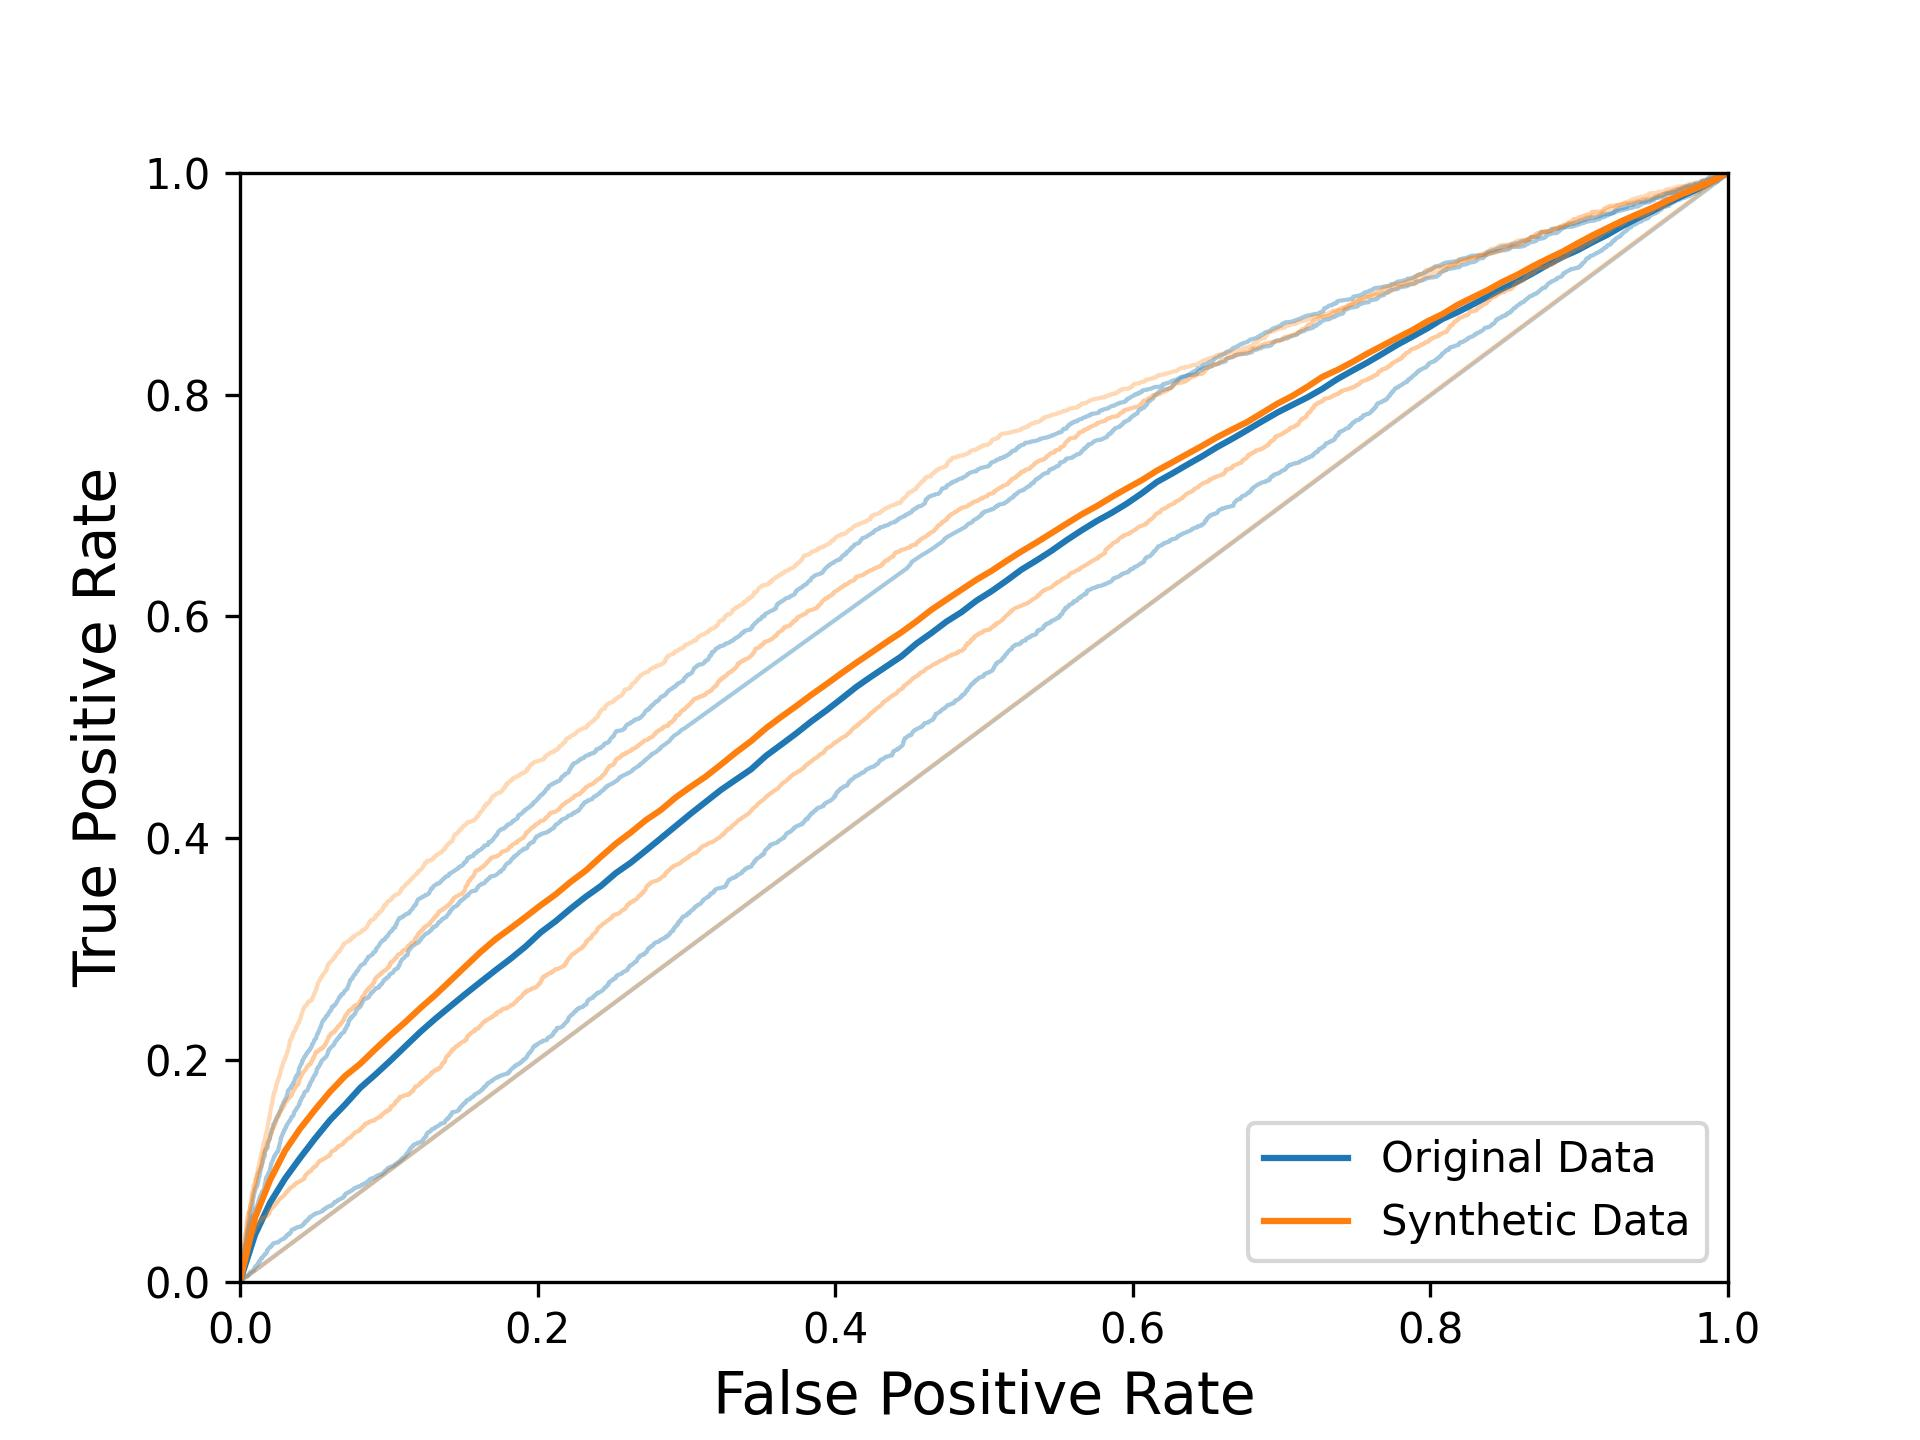
\includegraphics[width=0.7\textwidth]{Documents/ROC.jpg}
    \caption{The ROC curve of the developed machine learning models on the original and synthetic data. The bolder lines represent the average of different models under the two scenarios.}
    \label{fig:ROC}

\end{figure}

\begin{figure}
\centering
    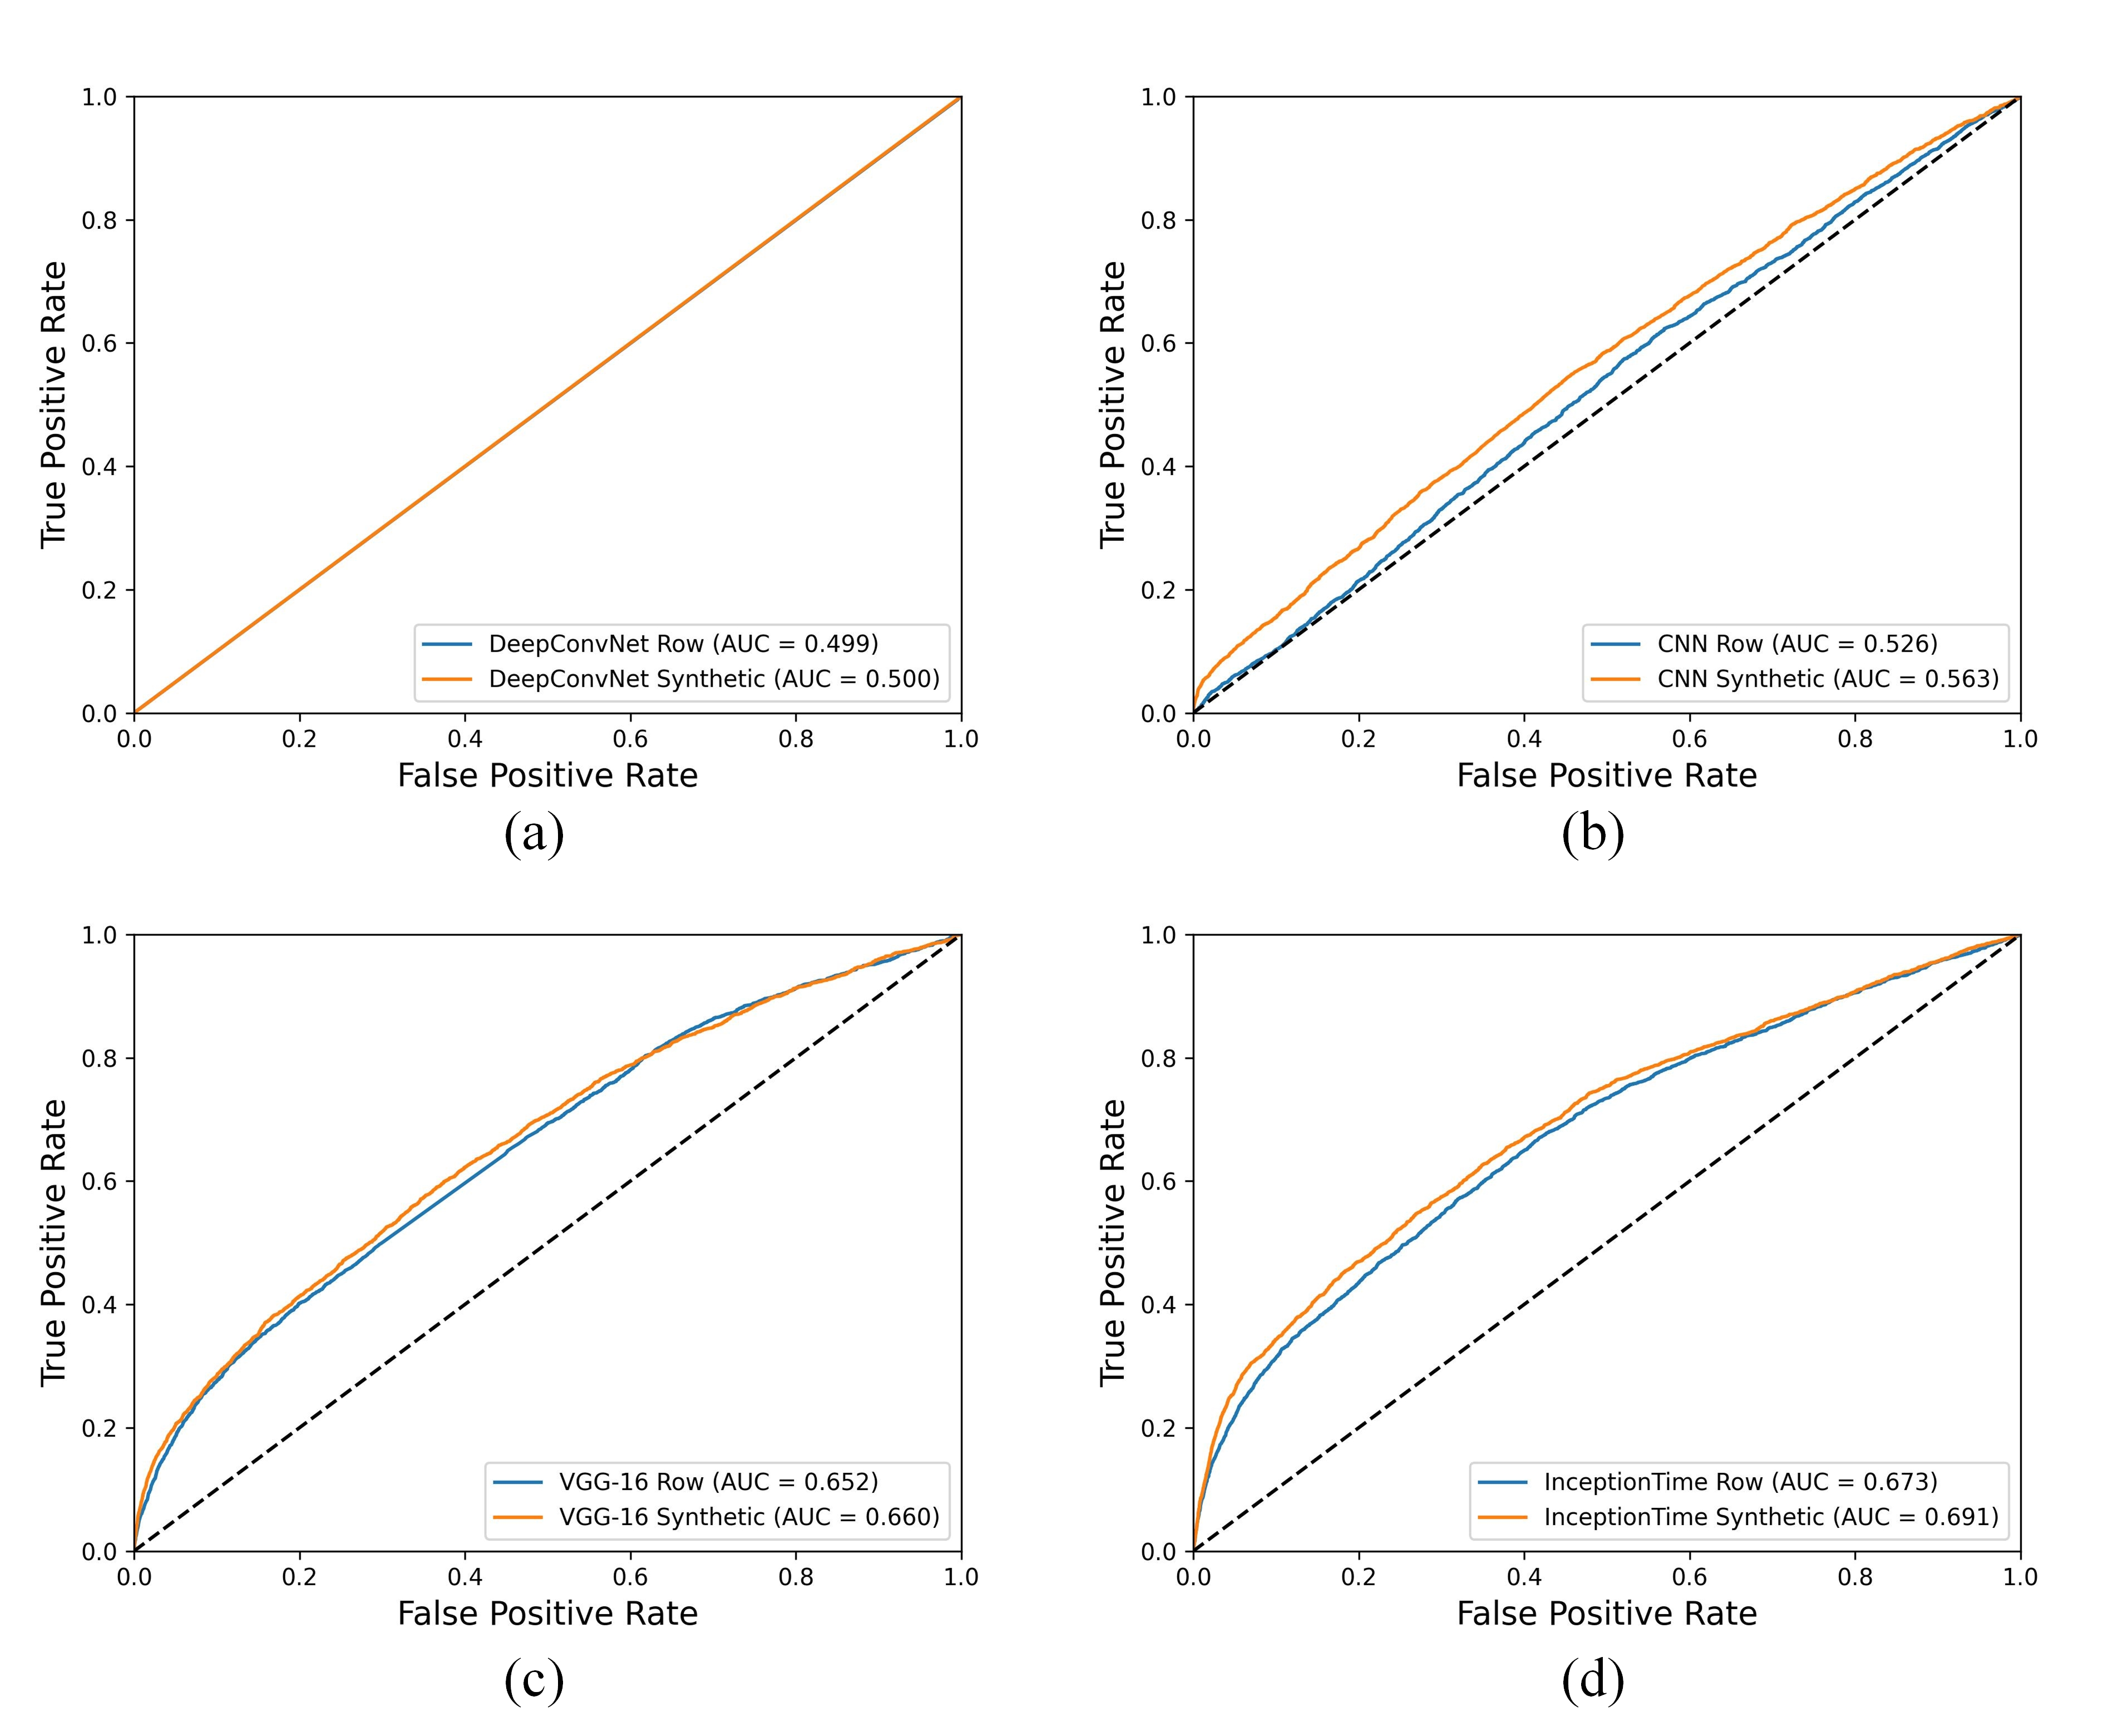
\includegraphics[width=0.7\textwidth]{Documents/ROCs.jpg}
    \caption{The individual ROC curves for the developed machine learning models. a) DeepConvNet, b) CNN, c) VGG-16, d) InceptionTime.}
    \label{fig:ROCs}

\end{figure}

\section{Discussion}
The conventional method for diagnosing heart murmurs involves auscultation, in which doctors depend on their listening abilities and clinical expertise to detect and analyze abnormal heart sounds. However, this approach is subjective and prone to variability, which can result in potential inaccuracies in diagnosis. As a result, researchers have been working to create more objective, dependable, and precise tools for evaluating heart murmurs, including automated decision support systems and machine learning algorithms.

\par Despite the promising potential of machine learning algorithms in heart murmur detection, one challenge that persists is the limited availability of high-quality data for training reliable and accurate models. Acquiring a sufficient amount of annotated heart sound recordings is crucial for developing effective algorithms. However, obtaining such data can be time-consuming and costly, as it requires the involvement of medical professionals to ensure accurate labeling. Furthermore, privacy concerns and ethical considerations surrounding the use of patient data can create additional barriers. 

\par Synthetic data can play a pivotal role in addressing the challenges associated with the limited availability of real-world data for training machine learning models in heart murmur detection. By generating artificial heart sound recordings that mimic the characteristics of real heart murmurs, large, diverse datasets can be created without the need for time-consuming data collection and manual annotation by medical professionals. Synthetic data can also help mitigate privacy concerns and ethical issues, as it does not involve the use of actual patient information.

\par While data collection for medical applications is typically aimed at capturing ideal recordings free of noise and environmental sounds, it is crucial to recognize that real-world scenarios often involve such imperfections.  One reason that machine learning models may not perform as well in real-world situations is their lack of exposure to noisy and imperfect data during the training process. Therefore, creating synthetic data that simulates the inherent noise of medical instruments and the background noise of a hospital setting can significantly enhance the generalizability of automated systems in real-world applications. By incorporating these realistic elements into the synthetic data, machine learning models can be trained to better handle the challenges of imperfect data, increasing their robustness and performance in actual clinical environments. 

\par The CirCor DigiScope PCG dataset, containing heart murmur recordings, was utilized for training machine learning models. We expanded the training dataset by generating synthetic data that mimicked a real hospital environment. Each heart sound was recorded with varying durations. To maximize the information extracted from each recording and increase the volume of training data for machine learning models, we divided the records into three-second segments. Since detecting heart murmur patterns in the time domain can be challenging, we applied the Mel spectrum to the segments, allowing the frequency domain images to be fed into the machine learning models. The implemented learning models included a simple CNN model developed from scratch, two pre-trained models with trainable fully-connected layers (DeepCocNet and VGG-16), and a time-series-based CNN model (InceptionTime). The latter model outperformed the others in terms of all performance metrics. Overall, the models trained on synthetic data demonstrated slightly better performance compared to those trained on the original data.

\subsection{Limitation}
Using synthetic data in healthcare comes with several limitations that need to be carefully considered. One of the limitations of synthetic data is the potential loss of subtle patterns and relationships present in real-world healthcare data. In our case study, the generated synthetic data may fail to capture the intricate complexities of the original data, at least in one of the time or frequency domains. For example, the synthetic instances are not easily distinguishable in the time domain, while they can preserve more the subtle patterns of the original data in the frequency domain.

\par The performance of the developed machine learning models is significantly influenced by the configuration and size of the dataset used for generating synthetic data. Modifying the SNR and SIR parameters of the synthetic data generator filters or adjusting the quantity of synthetic data used for training the machine learning models may lead to different results. Furthermore, due to the randomized nature of the synthetic data generator filters and the train-test split, different trials may yield varying outcomes. Therefore, it is crucial to consider conducting multiple trials using cross-validation techniques in future studies.

\par In this study, we evaluated four machine learning models, but other pre-trained or custom-developed models could potentially yield different results. Additionally, generating a large volume of synthetic data can be time-consuming and computationally expensive when training machine learning models. This necessitates ensuring that resource-rich settings are available to train the models over an adequate number of epochs.


\section{Conclusion}
A limited amount of training and validation data is often a bottleneck in the development of machine learning models, particularly in the healthcare domain. Gathering data can be time-consuming, expensive, and challenging to annotate, making it difficult to create reliable and generalizable machine learning models for specific tasks, such as heart murmur detection. This study aimed to address this issue by generating synthetic data that mimics a real hospital environment, in order to expand the training data for developing machine learning techniques. Four distinct machine learning models were designed to detect heart murmurs from PCG recordings with and without the generated synthetic data. The results indicated that augmenting the training set with synthetic data can potentially improve the performance of machine learning models.

\bibliographystyle{ieeetr}
\bibliography{ref}

\end{document}
